\documentclass[12pt,a4paper]{article}
\usepackage[pdftex]{graphicx}
\graphicspath{{Image/}}
\usepackage{epstopdf}
\usepackage{float}
\usepackage{amsmath}
\usepackage{mathtools}
\DeclarePairedDelimiter\abs{\lvert}{\rvert}
\DeclarePairedDelimiter\norm{\lVert}{\rVert}
\usepackage{esint}
\usepackage{amsfonts}
\usepackage{times}
\usepackage[top=.6 in, left=0.9in, right=0.9in]{geometry}
\usepackage{bbm}
\usepackage{dsfont}
\usepackage{enumerate}
\usepackage{titlesec}
\newcommand{\rn}{\mathbb{R}}
\newcommand{\E}{\mathbb{E}}
\newcommand{\Gn}{\mathbb{G}_{n}}
\newcommand{\G}{\mathbb{G}}
\newcommand {\tab}{\hspace{10 mm}}
\DeclareMathOperator*{\argmax}{arg\,max}
\DeclareMathOperator*{\argmin}{arg\,min}
\titleformat{\section}[block]{\large \it \filcenter}{}{0.5 ex}{}
\titleformat{\subsection}[block]{\small\it \filcenter}{}{0.5 em}{}
\titleformat{\subsubsection}[block]{\small\it \filcenter}{}{0.5 em}{}
\title{Empirical Methods in Economics\\\small{Assignment III}}
\date{Orville D. Mondal\\ $6^{th}$ of October, 2018\vspace{-3ex}}
\begin{document}
\maketitle
\begin{itemize}
\item The results of the estimation, for the four methods, are given in the table below. For the simplex method, I've used Matlab's \texttt{fminsearch} function, while for the quasi-newton implementations, I've used \texttt{fminunc}. It is of some comfort that the values of the coefficients do not change between different optimization routines.
\begin{table}[h]
\caption{Estimated coefficients}\vspace{2mm}
\centering
\begin{tabular}{c c c c c}
\hline \hline\vspace{2mm}
Coefficient &MLE (Simplex) &MLE (Quasi Newton) &NLS (lsqnonlin) &NLS (Simplex)\\
\hline
Constant&2.5339&2.5339&2.5126&2.5126\\
Age&-0.0323&-0.323&-0.0384&-0.0384\\
Years Married&0.1157&0.1157&0.1141&0.1141\\
Religiousness&-0.3540&-0.3540&-0.2796&-0.2796\\
Occupation&0.0798&0.0798&0.0676&0.0676\\
Self-rating of Marriage&-0.4094&-0.4094&-0.3698&-0.3698\\
\end{tabular}
\end{table}
\item In the above, it should be noted that \texttt{fminunc} is extremely sensitive to the initial point, when estimating MLE (not NLS). Also, during MLE, using \texttt{fminsearch} results in relatively slow convergence, requiring that one manually set the maximum number of iterations in the problem, or restart the evaluation at the point it breaks.
\item In terms of robustness to starting values, I'd rank Nelder-Mead over Quasi Newton methods. Timing considerations are slightly more interesting. The plot on the following page shows time taken till convergence, for a number of initial starting values. The initial points are chosen such that all methods converge (either themselves, or the area of the simplex, in the case of Nelder-Mead is negligibly small). To allow for a simple illustration, I am considering perturbations in a single dimension of the initial value, namely the first component. In all the estimations above, I have used a starting vector of \texttt{[3,0,0,0,0,0]}. The figure below shows the time till convergence for a hundred initial values of the form \texttt{[a,0,0,0,0,0]}, where \texttt{a} ranges from 2 to 4.
\item As can be seen, Nelder-Mead takes longer to converge than Quasi-Newton in the case of MLE. For NLS, however, Nelder-Mead performs better than the standard \texttt{nsqnonlin} function.
\end{itemize}
\begin{figure}[h!]
\centering
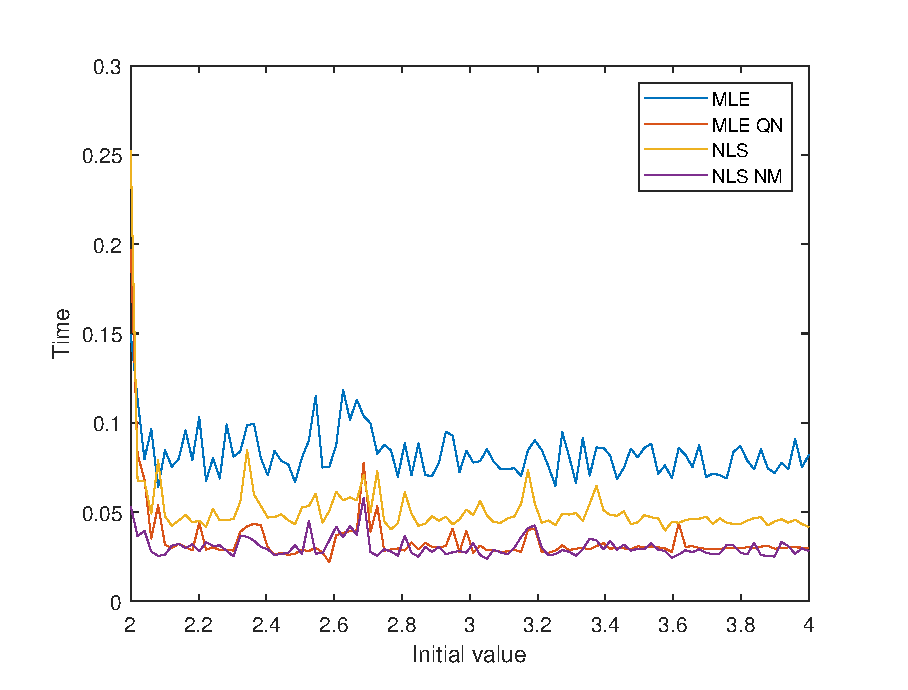
\includegraphics[width=0.9\textwidth]{fig1.eps}
\caption{Time taken for convergence in coefficients, for the four methods, in a neighbourhood of starting values.}
\end{figure}
\end{document} 